% ============================================
% ===== ANEXO  2: CREACIÓN DE CUENTA Y OBTENCIÓN DE TOKEN =====
% ============================================

\chapter{Crear cuenta y obtener token}
\label{anexo:crear-cuenta-token}
\section{Creación de la Cuenta}

Para la creación se puede hacer desde el inicio de sesión del DCD, que es el siguiente.

\begin{figure}[!h]
\begin{center}
\vspace*{0.3in}
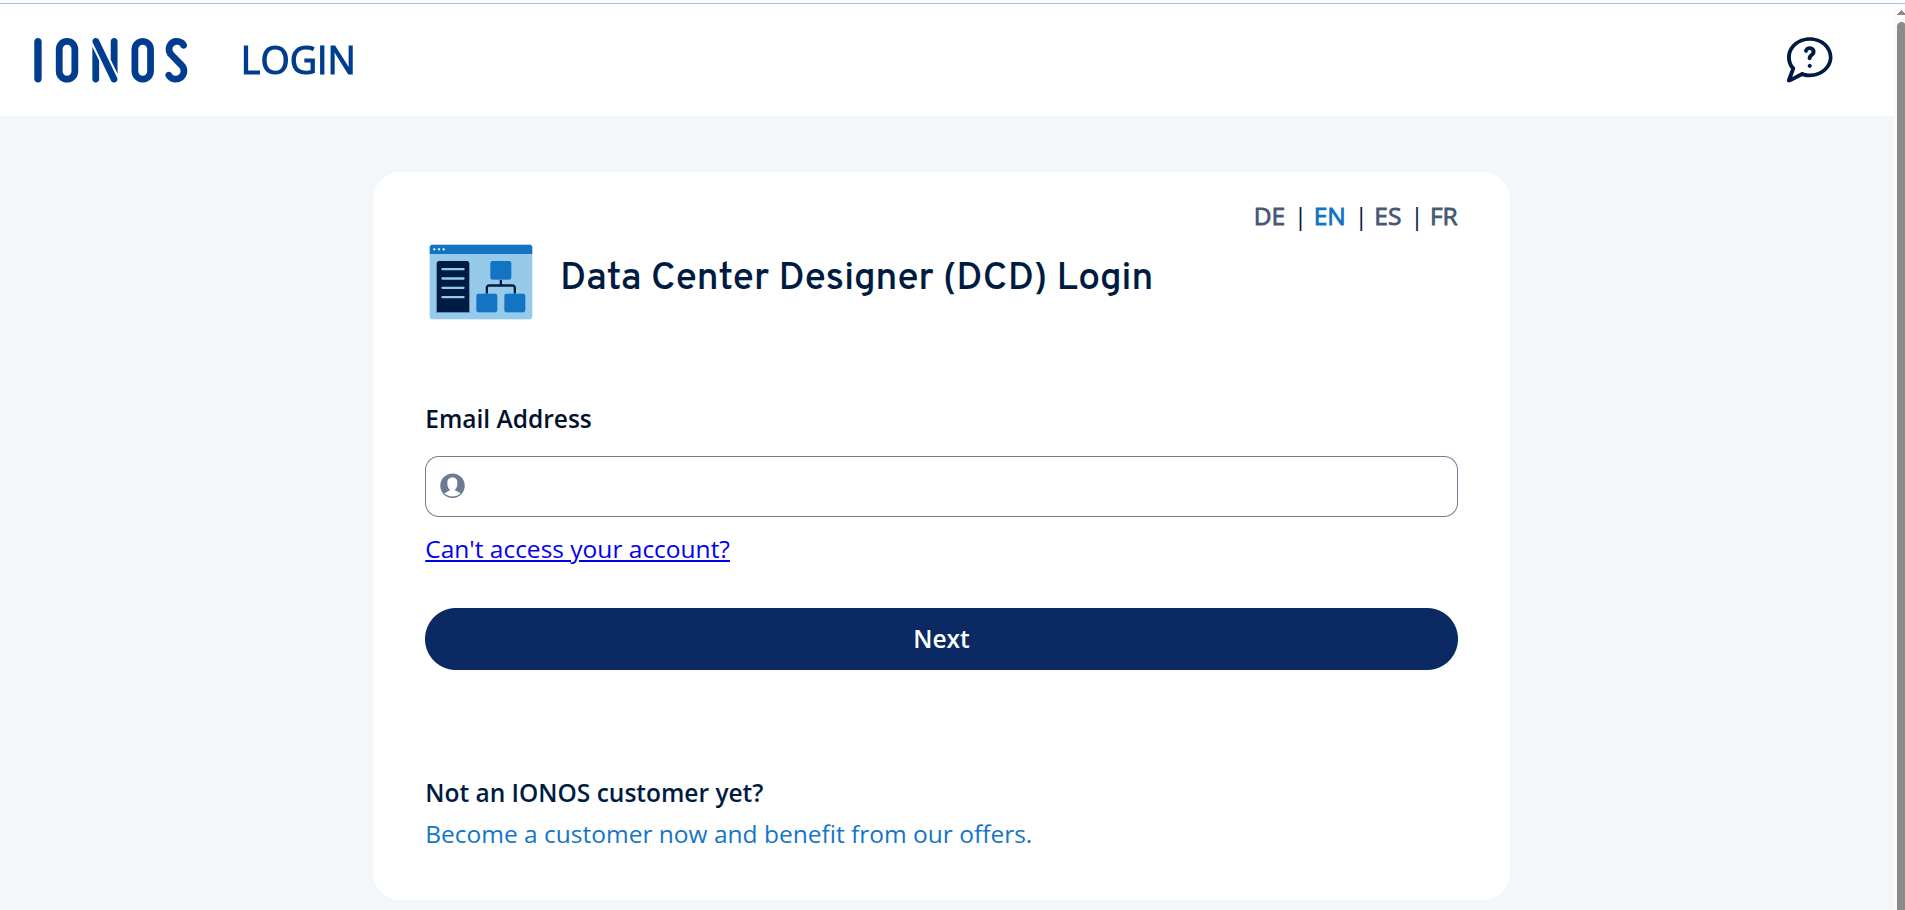
\includegraphics[width=10.5cm]{./imagenes/interfaz-InicioSesionDCD-1.png}
\caption*{Interfaz inicio sesión DCD IONOS Claud}
\end{center}
\end{figure}
Cuando se tenga cuenta solo hará falta añadir el correo en email address e iniciar sesión como es el estandar.
En el caso actual se debe dirigir a "\textit{Not an IONOS customer yet?}, dirgiendo este enlace a la web de creación de cuentas.

\begin{figure}[htb]
    \begin{center}
    \vspace*{0.3in}
    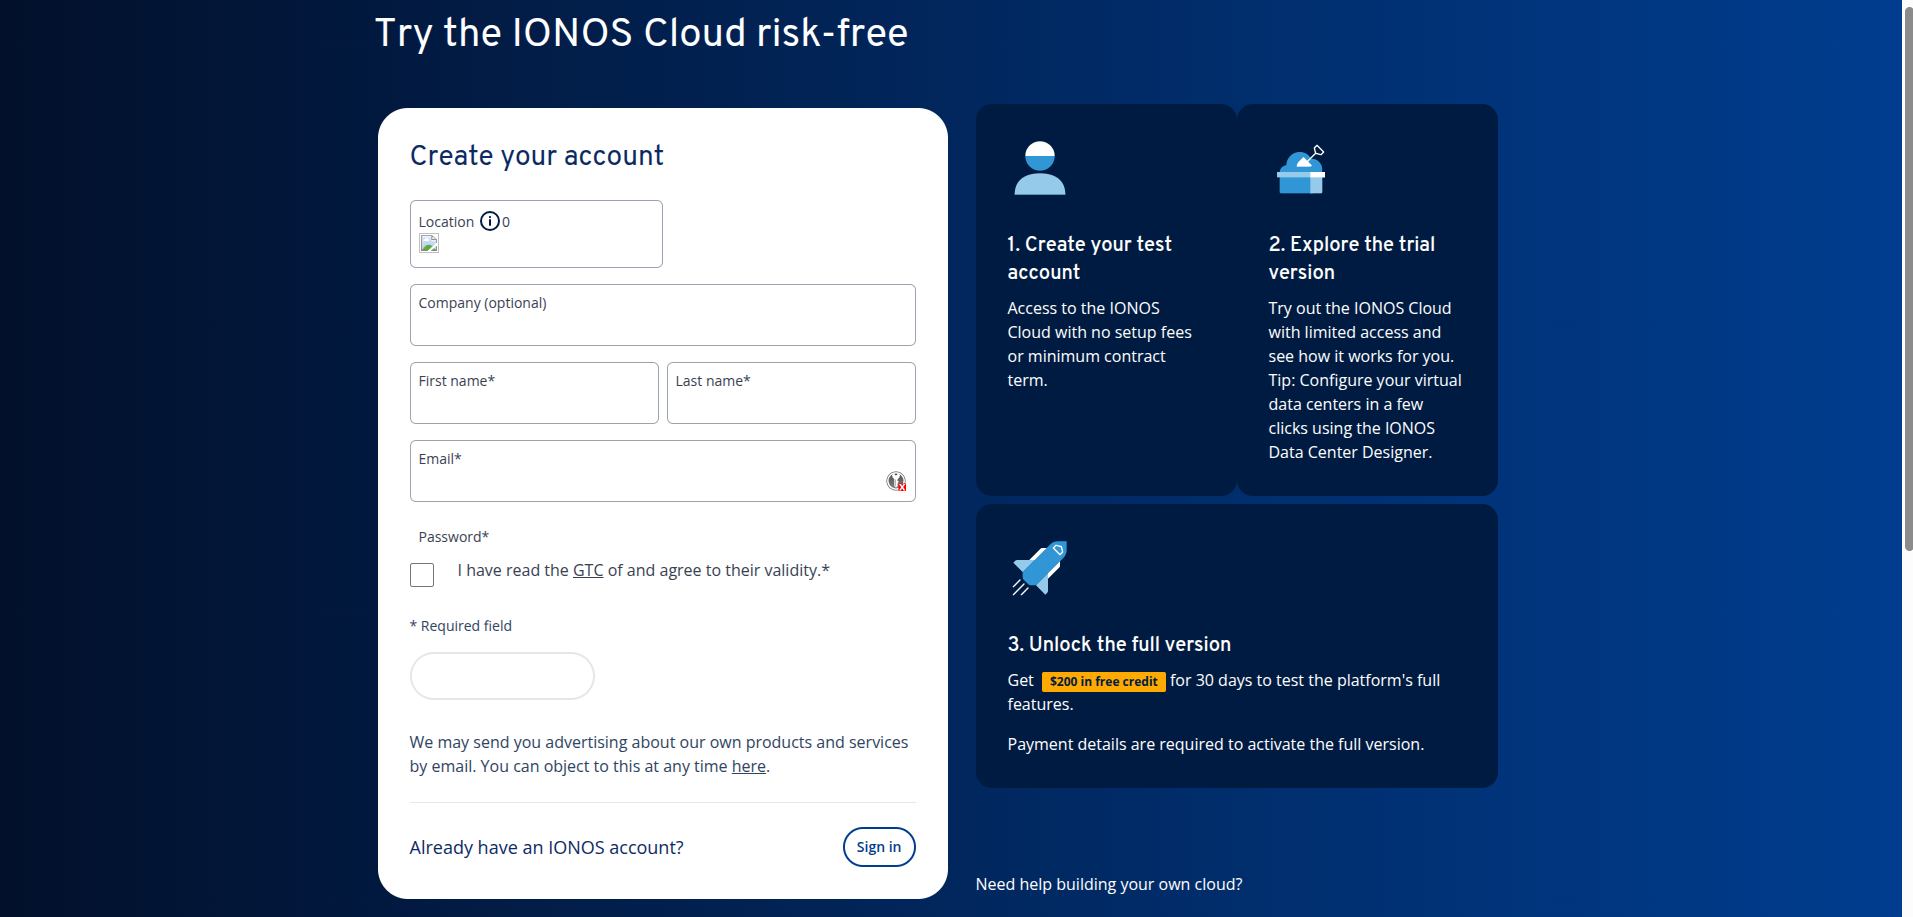
\includegraphics[width=10.5cm]{./imagenes/interfaz-InicioSesionDCD-2.png}
    \caption*{Crear cuenta IONOS Claud}
    \end{center}
\end{figure}

Como se puede ver en la imagen, lo unico que hay que hacer es añadir datos estandar y posteriormente aceptar sus políticas de privacidad.
Una vez creada la cuenta, se vuelve a la parte anterior y se inicia sesión con el correo al que se ha asociado la cuenta. Una ve iniciado se entrará en una pagina
similar a la mostrada actualmente. 

\begin{figure}[htb]
    \begin{center}
    \vspace*{0.3in}
    
\includegraphics[width=12.5cm]{interfaz-DCD-1.png}
    \caption*{Iterfaz inicio DCD IONOS Claud}
    \end{center}
\end{figure}

Una vez dentro ya se habra creado el contrato y se tendrá la cuenta, completando el primer paso.

\section{Obtener token}
Una vez dentro de la interfaz, se debe pinchar en "\textit{MANAGEMENT}" donde se desplegará un menú en el que se deberá seleccionar \textit{"Token Manager"}.
\begin{figure}[htb]
    \begin{center}
    \vspace*{0.3in}
    
\includegraphics[width=4.5cm]{interfaz-DCD-3.png}
    \caption*{Barra de gestión del DCD}
    \end{center}
\end{figure}
Una vez dentro, es muy intuitivo como generar un token, se debe seleccionar la duración de validez del token, esta dependerá del uso que se quiera dar a dicho token. Una vez creado se debe almacenar correctamente dicho token, debido a que es información valiosa y se debe llevar acabo un protocolo te protección para este.
\begin{figure}[htb]
    \begin{center}
    \vspace*{0.3in}
    
\includegraphics[width=10.5cm]{interfaz-DCD-tokens.png}
    \caption*{Interfaz de gestión de tokens}
    \end{center}
\end{figure}